% Credits are indicated where needed. The general idea is based on a template by Vel (vel@LaTeXTemplates.com) and Frits Wenneker.

\documentclass[11pt, a4paper]{article} % General settings in the beginning (defines the document class of your paper)
% 11pt = is the font size
% A4 is the paper size
% “article” is your document class

%----------------------------------------------------------------------------------------
%	Packages
%----------------------------------------------------------------------------------------

% Necessary
\usepackage[german,english]{babel} % English and German language 
\usepackage{booktabs} % Horizontal rules in tables 
% For generating tables, use “LaTeX” online generator (https://www.tablesgenerator.com)
\usepackage{comment} % Necessary to comment several paragraphs at once
\usepackage[utf8]{inputenc} % Required for international characters
\usepackage[T1]{fontenc} % Required for output font encoding for international characters

% Might be helpful
\usepackage{amsmath,amsfonts,amsthm} % Math packages which might be useful for equations
\usepackage{tikz} % For tikz figures (to draw arrow diagrams, see a guide how to use them)
\usepackage{tikz-cd}
\usetikzlibrary{positioning,arrows} % Adding libraries for arrows
\usetikzlibrary{decorations.pathreplacing} % Adding libraries for decorations and paths
\usepackage{tikzsymbols} % For amazing symbols ;) https://mirror.hmc.edu/ctan/graphics/pgf/contrib/tikzsymbols/tikzsymbols.pdf 
\usepackage{blindtext} % To add some blind text in your paper
\usepackage{graphicx}
\graphicspath{ {./images/} }


%---------------------------------------------------------------------------------
% Additional settings
%---------------------------------------------------------------------------------

%---------------------------------------------------------------------------------
% Define your margins
\usepackage{geometry} % Necessary package for defining margins

\geometry{
	top=2cm, % Defines top margin
	bottom=2cm, % Defines bottom margin
	left=2.2cm, % Defines left margin
	right=2.2cm, % Defines right margin
	includehead, % Includes space for a header
	%includefoot, % Includes space for a footer
	%showframe, % Uncomment if you want to show how it looks on the page 
}

\setlength{\parindent}{15pt} % Adjust to set you indent globally 

%---------------------------------------------------------------------------------
% Define your spacing
\usepackage{setspace} % Required for spacing
% Two options:
\linespread{1.5}
%\onehalfspacing % one-half-spacing linespread

%----------------------------------------------------------------------------------------
% Define your fonts
\usepackage[T1]{fontenc} % Output font encoding for international characters
\usepackage[utf8]{inputenc} % Required for inputting international characters

\usepackage{XCharter} % Use the XCharter font


%---------------------------------------------------------------------------------
% Define your headers and footers

\usepackage{fancyhdr} % Package is needed to define header and footer
\pagestyle{fancy} % Allows you to customize the headers and footers

%\renewcommand{\sectionmark}[1]{\markboth{#1}{}} % Removes the section number from the header when \leftmark is used

% Headers
\lhead{} % Define left header
\chead{\textit{}} % Define center header - e.g. add your paper title
\rhead{} % Define right header

% Footers
\lfoot{} % Define left footer
\cfoot{\footnotesize \thepage} % Define center footer
\rfoot{ } % Define right footer

%---------------------------------------------------------------------------------
%	Add information on bibliography
\usepackage{natbib} % Use natbib for citing
\usepackage{har2nat} % Allows to use harvard package with natbib https://mirror.reismil.ch/CTAN/macros/latex/contrib/har2nat/har2nat.pdf

% For citing with natbib, you may want to use this reference sheet: 
% http://merkel.texture.rocks/Latex/natbib.php

%---------------------------------------------------------------------------------
% Add field for signature (Reference: https://tex.stackexchange.com/questions/35942/how-to-create-a-signature-date-page)
\newcommand{\signature}[2][5cm]{%
  \begin{tabular}{@{}p{#1}@{}}
    #2 \\[2\normalbaselineskip] \hrule \\[0pt]
    {\small \textit{Signature}} \\[2\normalbaselineskip] \hrule \\[0pt]
    {\small \textit{Place, Date}}
  \end{tabular}
}
%---------------------------------------------------------------------------------
%	General information
%---------------------------------------------------------------------------------
\title{EE 308: Study of 400 KV Substation} % Adds your title
\author{Satyajeet Deshmukh (170002042)}    % Add your first and last name
 

\date{\small \today} % Adds the current date to your “cover” page; leave empty if you do not want to add a date

%---------------------------------------------------------------------------------
%	Define what’s in your document
%---------------------------------------------------------------------------------

\begin{document}


% If you want a cover page, uncomment "%---------------------------------------------------------------------------------
% Cover page
%---------------------------------------------------------------------------------

% Here are more templates for other cover pages: https://www.latextemplates.com/cat/title-pages

% This example is based on this cover page example: https://www.latextemplates.com/template/academic-title-page

\begin{titlepage} % Starts new environment where the page number is not displayed and the count starts at 1 for the next page

%------------------------------------------------
%	Institutional information
%------------------------------------------------
	
\begin{minipage}{0.4\textwidth} % Begins new environment (like a text box)
    \begin{flushleft} % Sets environment on the left side of the paper
    \large
    University of XX\\ % Add your institution
    Chair of Political Science IV\\ % Add the chair
    Fall 2018\\ % Add term
    COURSE TITLE\\ % Add course title
    Supervisor: NAME % Add instructor/supervisor name 
    \end{flushleft}
\end{minipage}
	
\vspace*{2in} % Adds some space in-between
	
\center % Centre everything on the page

%------------------------------------------------
%	Main part
%------------------------------------------------
	
{\huge\bfseries TITLE OF YOUR PAPER}\\[0.4cm] % Add your paper title 
{\large\today}\\[0.4cm] % Add date (current day)
FIRSTNAME LASTNAME % Add your name
	
\vfill % Adds additional space

%------------------------------------------------
%	General information about the author
%------------------------------------------------

\vfill % Adds additional space

Your contact info \\ % Add your contact info
Your Program \\ % Add info about your program
Semester you are enrolled \\ % Add info about your semester

\vfill % Adds additional space

%------------------------------------------------
%	Word count
%------------------------------------------------

\vfill % Adds additional space
	
Word count: XXXX % To indicate the word count
% How to check words in a LaTeX document: https://www.overleaf.com/help/85-is-there-a-way-to-run-a-word-count-that-doesnt-include-latex-commands
	

	
\end{titlepage}" and uncomment "\begin{comment}" and "\end{comment}" to comment the following lines
%%---------------------------------------------------------------------------------
% Cover page
%---------------------------------------------------------------------------------

% Here are more templates for other cover pages: https://www.latextemplates.com/cat/title-pages

% This example is based on this cover page example: https://www.latextemplates.com/template/academic-title-page

\begin{titlepage} % Starts new environment where the page number is not displayed and the count starts at 1 for the next page

%------------------------------------------------
%	Institutional information
%------------------------------------------------
	
\begin{minipage}{0.4\textwidth} % Begins new environment (like a text box)
    \begin{flushleft} % Sets environment on the left side of the paper
    \large
    University of XX\\ % Add your institution
    Chair of Political Science IV\\ % Add the chair
    Fall 2018\\ % Add term
    COURSE TITLE\\ % Add course title
    Supervisor: NAME % Add instructor/supervisor name 
    \end{flushleft}
\end{minipage}
	
\vspace*{2in} % Adds some space in-between
	
\center % Centre everything on the page

%------------------------------------------------
%	Main part
%------------------------------------------------
	
{\huge\bfseries TITLE OF YOUR PAPER}\\[0.4cm] % Add your paper title 
{\large\today}\\[0.4cm] % Add date (current day)
FIRSTNAME LASTNAME % Add your name
	
\vfill % Adds additional space

%------------------------------------------------
%	General information about the author
%------------------------------------------------

\vfill % Adds additional space

Your contact info \\ % Add your contact info
Your Program \\ % Add info about your program
Semester you are enrolled \\ % Add info about your semester

\vfill % Adds additional space

%------------------------------------------------
%	Word count
%------------------------------------------------

\vfill % Adds additional space
	
Word count: XXXX % To indicate the word count
% How to check words in a LaTeX document: https://www.overleaf.com/help/85-is-there-a-way-to-run-a-word-count-that-doesnt-include-latex-commands
	

	
\end{titlepage}

%\begin{comment}
\maketitle % Print your title, author name and date; comment if you want a cover page 
%\end{comment}

\begin{center}
    Source Code: https://www.overleaf.com/read/zsfbpmyscfwm
\end{center}

%----------------------------------------------------------------------------------------
% Introduction
%----------------------------------------------------------------------------------------
\setcounter{page}{1} % Sets counter of page to 1

\section{Foreword}
As this is just a study, any originality should not expected. I have tried to phrase things as much as I can where there were conceptual ideas involved, and add in inferences. Direct quotes have been used appropriately and credits have been given to the authors. Direct quotes were inevitable as the information uses certain jargon which even if I paraphrase just looked the same. Paraphrasing will still count as Metaphor Plagiarism if not credited properly. I have tried to cover the main conceptual ideas while skipping over safety, insulation and regulations parts and focused on how to design.

\section{Introduction} % Add a section title
\subsection{Definition: Substation} % Add a subsection
"Substations are the points in the power network where transmission lines and distribution feeders are connected together through circuit breakers or switches via busbars and transformers. This allows for the control of power flows in the network and general switching operations for maintenance purposes." \citep[Chap.3]{book1}

This is a very broad definition. We shall further look into more elaborate descriptions for a better understanding.

\subsection{Basics Design Aspects of Substations}
"Substations are power stations that include power transformers, potential or voltage transformers, current transformers, electrical bus, breakers, switches, and so on.  A substation is a station that includes a power transformer for either stepping up or stepping down the supply voltage depending on whether it is a generating substation or transmission/distribution substation. Generating substations step up the voltage from the generator’s lower voltage to a higher voltage which is more economical for transmitting electric power over longer distances with less power losses caused by the impedance of transmission lines. Transmission substations take the incoming higher voltage from transmission lines and step them down to a lower voltage for distribution systems, which is in preparation for end user customers."

The 400 KV transmission substations will be used to distribute the power to lower voltage distribution substations which it will receive from higher voltage generation substations. 

"Power Substations are filled with large and very expensive equipment. A power utilities’ greatest expense in substations is the power transformer. Other items and equipment involved in designing substations which are less expensive than power transformers are: circuit breakers, potential/current transformers, electric bus, steel structures, foundations, control house, protection \& controls (P\&C), relaying/IEDs, SCADA, control cables, fencing, grounding, real estate, etc."

See reference of \citet{basics-of-power-substations}

\subsection{Indian Power Grid} % Add another subsection
The nominal Extra High Voltage lines in vogue are ± 800 kV HVDC \& 765 kV, 400 kV, 230/220 kV, 110 kV and 66 kV AC lines. We can calculate that 36\% of the total load is handled by 400 KV substations in India. See exec report of \citet{execsummary2020} in references.

%----------------------------------------------------------------------------------------
% Literature
%----------------------------------------------------------------------------------------

\section{Designing a new Substation}

\subsection{Reading the guidelines}

Before starting the load calculations it is important to go through the regional limits of voltage levels.  

"Normal thermal ratings and normal voltage limits represent equipment limits
that can be sustained on continuous basis. Emergency thermal ratings and emergency voltage limits represent equipment limits that can be tolerated for a relatively short time which may be one hour to two hour depending on design of the equipment." 

They state nominal rating as 400 KV rms. Maximum as 420 and minimum as 380 under normal operating conditions. Emergency ratings are maximum at 420 and minimum at 372. 

"The system shall be planned based on one or more of the following power
system studies, as per requirements:
i) Power Flow Studies
ii) Short Circuit Studies
iii) Stability Studies (including transient stability and voltage stability)
iv) EMTP studies (for switching / dynamic over-voltages, insulation
coordination, etc) "

Going through them  all is beyond the scope for this study. We shall take a peek into the power flow studies as it is simple and essential to understand.

For more information see \citet{manualontransmission}.
 
\subsection{Load Flow Power Studies}

The next steps are to calculate the total power coming in from the generators. Then balance it with the power going out for distribution and power being used for the maintenance of the substation itself.

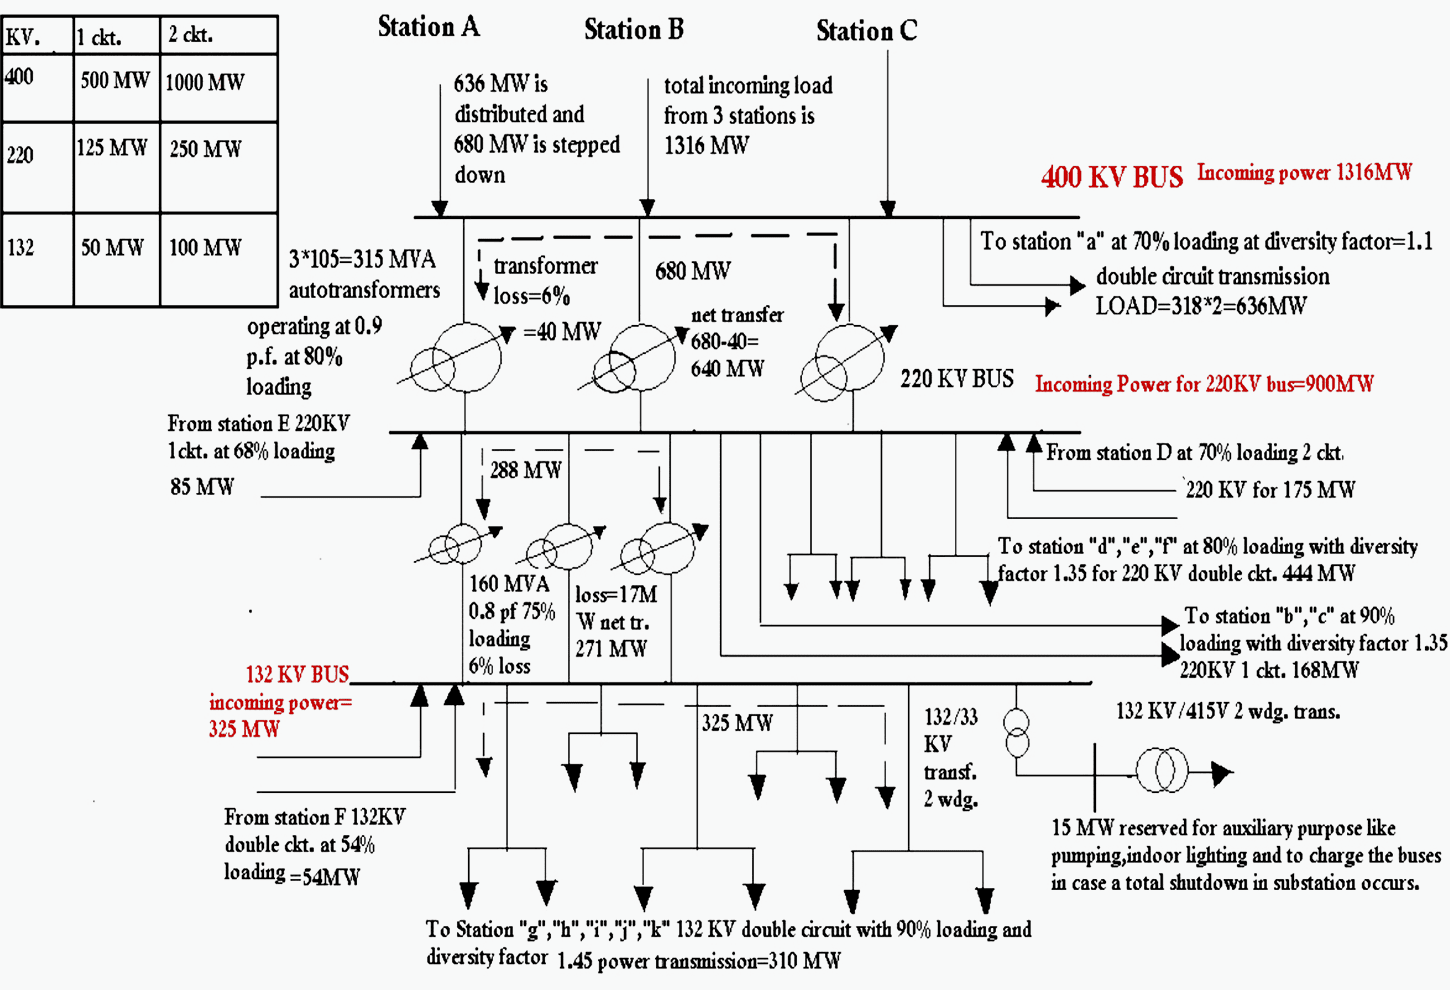
\includegraphics[scale=0.3]{substation-load-distribution-diagram}

Figure: Substation load distribution diagram from \citet{400kVSubstationDesign}

In the figure we can see how an elementary analysis of power is performed. Though it is not sufficient. We will need to use computer models and simulations to ensure that our system is stable and following the regulations set by the boards.

\subsection{Selection of Site}
\citet{400kVSubstationDesign} describes the selection of site in detail. I will cover it briefly here in my own words.

Selection of the site for the substation is one of the most important activities which requires meticulous planning, technical knowledge, understanding of geography, environment, economics, and social aspects.

\begin{itemize}
  \item The site should be as close to the load centre as possible
  \item It should be ideally rectangular for proper fitting of bus bars, and have an area of 20 hectares for a 400 KV substation.
  \item Preferably levelled already to save costs in levelling.
  \item It should be away from any present human settlement, or activity like dumping grounds, and not in a zone of future development activities.
  \item There should be good road access to the site.
  \item There should not be an airport in vicinity and  it should be above the flood levels so that water doesn't fill up.
\end{itemize}

\subsection{Substation Configurations}

Each transmission substation consists of the following key elements:

\begin{itemize}
    \item Incomers: Feed power into the substation.
    \item Bus bars: Connect the different circuits together.
    \item Bus coupler: Allow different bus bars to be connected together.
    \item Feeders: Take power out of the substation.
\end{itemize}

They can be connected in various ways according to the requirement of the project for load and local conditions, flexibility of operations, maintenance and safety, and economic considerations like cost.

Common configurations are as follow:
\begin{itemize}
    \item Single bus bar substation: Single incomer is connected to single bus bar which distributes power to multiple feeders.
    \item Split bus bar substation: Two incomers are connected to two separate bus bars. In normal configurations they both keep supply only their own bus bar. If one one of the incomer fails causing an emergency, the two busbars are coupled and energized by only one incomer.
    \item Double bus bar station: There are two incomers and four busbars. We can change which bus bar the feeder is connected to easily.This provides huge flexibility and convenience while doing maintenance.
    \item Double main and auxiliary bus bar: This is an improvement over the double bus bar by providing Auxiliary bus, bus coupler breaker and Auxiliary bus isolators which are used during maintenance.
    \item Ring: "The ring bus bar offers increased security compared to the single bus bar arrangement since alternative power flow routes around the ring bus bar are available." 
    
    Section material is based on readings from \citet{book1}
    
\end{itemize}

\subsection{Substation Auxiliary Power Supplies}

Every substations includes auxiliary power supplies which may consist of batteries which power DC and AC circuits via circuitry. Batteries are charged regularly using the some of the incoming power from generators. "AC power is required for substation building small power, lighting, heating and ventilation,
some communications equipment, switchgear operating mechanisms, anticondensation heaters and motors. 
DC power is used to feed essential services such as circuit breaker trip coils and associated relays, supervisory control and data acquisition and communications equipment."
from \citet{book1}

\section{Conclusion}

Thus, we have seen 400 KV substations that are used for transmission can range from simple to complex. They may use simple bus bar designs or may be loaded with sophisticated protection and control equipment. 

%----------------------------------------------------------------------------------------
% Bibliography
%----------------------------------------------------------------------------------------
\newpage % Includes a new page

\pagenumbering{roman} % Changes page numbering to roman page numbers
%\bibliography{literature}

\bibliography{literature.bib} % Add the filename of your bibliography
\bibliographystyle{apsr} % Defines your bibliography style

% For citing, please see this sheet: http://merkel.texture.rocks/Latex/natbib.php


%---------------------------------------------------------------------------------

\end{document}
